Los puntos 1.3 y 1.4 se implementaron en el notebook \texttt{punto\_1\_5\_qiskit.ipynb}, con las
herramientas que se usan en el curso de IBM Quantum Learning (\emph{Basics of quantum
information}): \texttt{Statevector} para los estados puros, \texttt{DensityMatrix} para los
proyectores y los estados mixtos, y circuitos de \texttt{QuantumCircuit} que se corren con el
\texttt{StatevectorSampler} para simular mediciones. Las funciones reciben $\alpha$ y $\beta$
cualesquiera; en este documento se reportan los resultados para el estado de los puntos 1.3 y
1.4,
\[
  \ket\psi=\tfrac{\sqrt3}{2}\ket0+\tfrac{i}{2}\ket1 ,
\]
y al final del notebook se repiten todas las comprobaciones con $200$ estados, valores de $\tau$,
$\eta$ y $p$ elegidos al azar.

\paragraph{Probabilidades exactas y frecuencias.}
Las probabilidades exactas se calculan con la regla de Born, que en Qiskit es el método
\texttt{probabilities\_dict()}: para un \texttt{Statevector} da $|\alpha|^2$ y $|\beta|^2$, y
para una \texttt{DensityMatrix} da la diagonal de la matriz. Para las mediciones simuladas se
arma un circuito de un qubit que prepara el estado con \texttt{initialize} y lo mide en la base
computacional, y se corre $N=4000$ veces. La frecuencia del resultado $0$ es una proporción
muestral, así que su desviación estándar es
\[
  \sqrt{\frac{P(0)\bigl(1-P(0)\bigr)}{N}}=\sqrt{\frac{0.75\cdot0.25}{4000}}\approx0.007 ,
\]
y las diferencias entre las frecuencias y las probabilidades exactas deben ser de ese orden.

%======================================================================
\subsection*{(a) Construcción de $\ket{\psi'}$ y $\eta$}
%======================================================================

La función \texttt{construir\_psi\_prima} aplica las fórmulas del punto 1.3,
\[
  \alpha'=-e^{-i\eta}\alpha,\qquad \beta'=e^{-i\eta}e^{i\tau}\beta,\qquad c=\beta\,(1+e^{i\tau}),
\]
y devuelve un error si $\beta=0$ (no hay solución) o si $\tau=\pm\pi$ (daría $c=0$). Se
probaron las tres soluciones del ejemplo del punto 1.3 con $\eta=0$ y una con $\eta=1$:

\begin{center}
\renewcommand{\arraystretch}{1.3}
\begin{tabular}{lcccc}
  Estado & $P(0)$ exacta & frecuencia de $0$ & $P(1)$ exacta & frecuencia de $1$\\\hline
  $\ket\psi$ & $0.75$ & $0.7555$ & $0.25$ & $0.2445$\\
  $\ket{\psi'}$, $\tau=0$ & $0.75$ & $0.7452$ & $0.25$ & $0.2547$\\
  $\ket{\psi'}$, $\tau=\frac\pi2$ & $0.75$ & $0.7418$ & $0.25$ & $0.2582$\\
  $\ket{\psi'}$, $\tau=-\frac\pi2$ & $0.75$ & $0.7620$ & $0.25$ & $0.2380$\\
  $\ket{\psi'}$, $\tau=0$, $\eta=1$ & $0.75$ & $0.7570$ & $0.25$ & $0.2430$
\end{tabular}
\end{center}

Todas las $\ket{\psi'}$ tienen exactamente las probabilidades de $\ket\psi$, y las frecuencias
quedan a menos de dos desviaciones estándar de ellas. Luego se calculó
$\ket\psi+e^{i\eta}\ket{\psi'}$, se normalizó y se comparó con $\ket1$ con el método
\texttt{equiv}, que dice si dos estados son iguales salvo fase global:

\begin{center}
\renewcommand{\arraystretch}{1.3}
\begin{tabular}{lccccc}
  Solución & $\ket\psi+e^{i\eta}\ket{\psi'}$ & norma & $|c|$ & ¿es $\ket1$ salvo fase? & frecuencia de $1$\\\hline
  $\tau=0$ & $(0,\ i)$ & $1$ & $1$ & sí & $1$\\
  $\tau=\frac\pi2$ & $(0,\ -0.5+0.5i)$ & $0.7071$ & $0.7071$ & sí & $1$\\
  $\tau=-\frac\pi2$ & $(0,\ 0.5+0.5i)$ & $0.7071$ & $0.7071$ & sí & $1$\\
  $\tau=0$, $\eta=1$ & $(0,\ i)$ & $1$ & $1$ & sí & $1$
\end{tabular}
\end{center}

La coordenada de $\ket0$ de la suma es $0$ en todos los casos, la norma de la suma es $|c|$
porque la suma es $c\ket1$, y al medir el estado normalizado solo se obtiene $1$. Los valores de
$c$ son los mismos de la tabla del punto 1.3. La solución con $\eta=1$ da la misma suma que con
$\eta=0$, porque $\eta$ solo compensa la fase global con la que se escribe $\ket{\psi'}$.

%======================================================================
\subsection*{(b) El estado mixto $p\rho+(1-p)\rho'$}
%======================================================================

Con la solución de $\tau=0$, $\ket{\psi'}=-\frac{\sqrt3}{2}\ket0+\frac{i}{2}\ket1$, se construyeron
$\rho$ y $\rho'$ con \texttt{DensityMatrix}, que calcula el proyector $\ket\psi\bra\psi$ a partir
del ket, y las mezclas $\rho_p=p\rho+(1-p)\rho'$ para $p=0,\frac14,\frac12,\frac34,1$. Las matrices
que se obtienen son las del punto 1.4; por ejemplo, para $p=\frac14$,
\[
  \rho_{1/4}=\begin{pmatrix}0.75 & 0.2165\,i\\ -0.2165\,i & 0.25\end{pmatrix},
\]
que coincide con $\rho_p$ del punto 1.4 para $p=\frac14$, pues
$-(2p-1)\frac{\sqrt3}{4}=\frac{\sqrt3}{8}\approx0.2165$.

Para simular las mediciones de la mezcla se usó lo que significa un estado mixto: en cada
medición el qubit está en $\ket\psi$ con probabilidad $p$ y en $\ket{\psi'}$ con probabilidad
$1-p$. Por eso, de las $N$ mediciones, el número que se hace con $\ket\psi$ es una variable
binomial con parámetros $N$ y $p$. Se generó ese número, se corrieron esas mediciones con el
circuito de $\ket\psi$ y las demás con el de $\ket{\psi'}$, y se juntaron los conteos:

\begin{center}
\renewcommand{\arraystretch}{1.3}
\begin{tabular}{ccccc}
  $p$ & $P(0)$ exacta & frecuencia de $0$ & $P(1)$ exacta & frecuencia de $1$\\\hline
  $0$ & $0.75$ & $0.7635$ & $0.25$ & $0.2365$\\
  $\frac14$ & $0.75$ & $0.7560$ & $0.25$ & $0.2440$\\
  $\frac12$ & $0.75$ & $0.7642$ & $0.25$ & $0.2358$\\
  $\frac34$ & $0.75$ & $0.7380$ & $0.25$ & $0.2620$\\
  $1$ & $0.75$ & $0.7505$ & $0.25$ & $0.2495$
\end{tabular}
\end{center}

Para todo $p$ las probabilidades exactas son las de $\ket\psi$, como se mostró en el punto 1.4, y
las frecuencias quedan cerca de ellas: la diferencia más grande, en $p=\frac12$, es de unas
$2.1$ desviaciones estándar.

%======================================================================
\subsection*{(c) Vectores de Bloch}
%======================================================================

Los vectores se calcularon con las fórmulas del punto 1.4, que leen el punto de la esfera de las
entradas de la matriz,
\[
  r_x=2\,\bigl(\text{parte real de }\rho_{10}\bigr),\qquad
  r_y=2\,\bigl(\text{parte imaginaria de }\rho_{10}\bigr),\qquad
  r_z=\rho_{00}-\rho_{11},
\]
y se compararon con la lectura \emph{r} que muestra el widget del punto 1.2 para cada estado
puro (las capturas del punto 1.3):

\begin{center}
\renewcommand{\arraystretch}{1.3}
\begin{tabular}{lccc}
  Estado & Qiskit & Widget & $|\vec r|$\\\hline
  $\ket\psi$ & $(0,\ 0.866,\ 0.5)$ & $(0,\ 0.866,\ 0.5)$ & $1$\\
  $\ket{\psi'}$, $\tau=0$ & $(0,\ -0.866,\ 0.5)$ & $(0,\ -0.866,\ 0.5)$ & $1$\\
  $\ket{\psi'}$, $\tau=\frac\pi2$ & $(0.866,\ 0,\ 0.5)$ & $(0.866,\ 0,\ 0.5)$ & $1$\\
  $\ket{\psi'}$, $\tau=-\frac\pi2$ & $(-0.866,\ 0,\ 0.5)$ & $(-0.866,\ 0,\ 0.5)$ & $1$\\
  estado final $\ket1$ & $(0,\ 0,\ -1)$ & $(0,\ 0,\ -1)$ & $1$\\\hline
  $\rho_p$, $p=0$ & $(0,\ -0.866,\ 0.5)$ & -- & $1$\\
  $\rho_p$, $p=\frac14$ & $(0,\ -0.433,\ 0.5)$ & -- & $0.6614$\\
  $\rho_p$, $p=\frac12$ & $(0,\ 0,\ 0.5)$ & -- & $0.5$\\
  $\rho_p$, $p=\frac34$ & $(0,\ 0.433,\ 0.5)$ & -- & $0.6614$\\
  $\rho_p$, $p=1$ & $(0,\ 0.866,\ 0.5)$ & -- & $1$
\end{tabular}
\end{center}

Los vectores de los estados puros coinciden con los del widget, que muestra tres decimales. El
widget solo representa estados puros, así que para las mezclas la comparación se hace con los
valores calculados en el punto 1.4, $\vec r_p=\bigl(0,(2p-1)\frac{\sqrt3}{2},\frac12\bigr)$, que
dan los mismos números. Todos los estados, salvo el final, tienen $r_z=0.5$: los estados puros
están en el paralelo de $\ket\psi$ ($|\vec r|=1$) y las mezclas con $0<p<1$ están en la cuerda
que une $\ket{\psi'}$ con $\ket\psi$, dentro de la esfera ($|\vec r|<1$). La
figura~\ref{fig:15-bloch} compara el dibujo de Qiskit con la figura del punto 1.4, que muestra la misma cuerda.

\begin{figure}[htbp]
\centering
\begin{minipage}{0.44\linewidth}\centering
  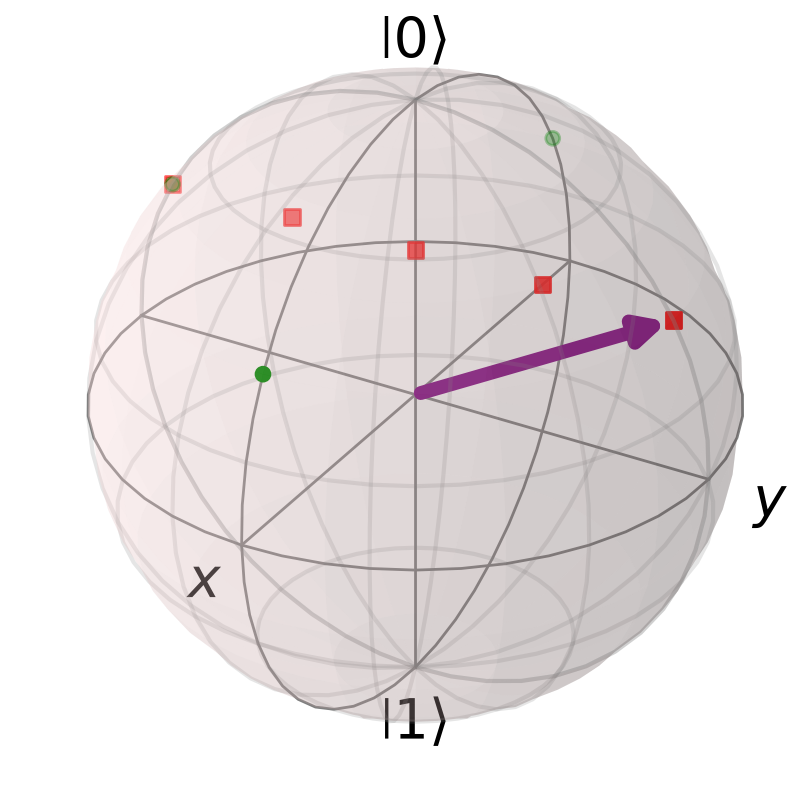
\includegraphics[width=\linewidth]{Imágenes/p15_bloch_qiskit.png}\\
  {\footnotesize Qiskit}
\end{minipage}\hspace{0.04\linewidth}
\begin{minipage}{0.44\linewidth}\centering
  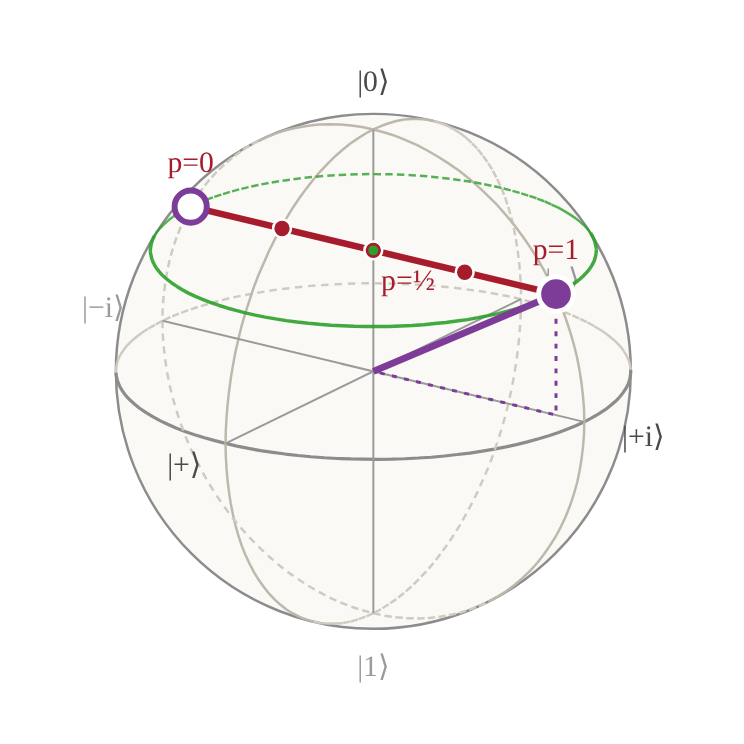
\includegraphics[width=\linewidth]{Imágenes/p14_mezcla_tau0.png}\\
  {\footnotesize Figura del punto 1.4}
\end{minipage}
\caption{A la izquierda, la esfera de Bloch dibujada con la clase \texttt{Bloch} de Qiskit: el
vector de $\ket\psi$ (morado), las tres soluciones $\ket{\psi'}$ del punto 1.3 (verde) y las
mezclas $\rho_p$ con la solución de $\tau=0$ (rojo). A la derecha, la figura del punto 1.4 con
la misma cuerda, porque el widget solo muestra estados puros. En las dos, los puntos de las mezclas quedan sobre el segmento horizontal entre
$\ket{\psi'}$ y $\ket\psi$, a altura $0.5$.}
\label{fig:15-bloch}
\end{figure}
